\newpage
\section {Билет 10. Методы обеспечения отказоустойчивости. RAID, распределенное хранение данных, виды и репликаций.}
\subsection {RAID}
RAID (Redundant Array of Independent Disks) - технология повышения отказоустойчивости и производительности дисковой подсистемы. Основная идея технологии заключается в распределении информации по массиву дисков с вычислением контрольных сумм. Поэтому в случае выхода из строя одного диска данные могут быть восстановлены с помощью информации, находящейся на других дисках. 
Выделяют несколько уровней (типов) RAID.

RAID 0. \\
Информация разбивается на блоки данных $A_{i}$ фиксированной длины и записывается на несколько дисков поочередно. На картинке приведен пример, с двумя дисками, но логически они составляют один диск. В этом подходе, при выходе из строя одного диска, информацию, которая на нем, хранилась никак не восстановить.

\begin{figure}[h!]
\begin{minipage}[h]{0.49\linewidth}
\center{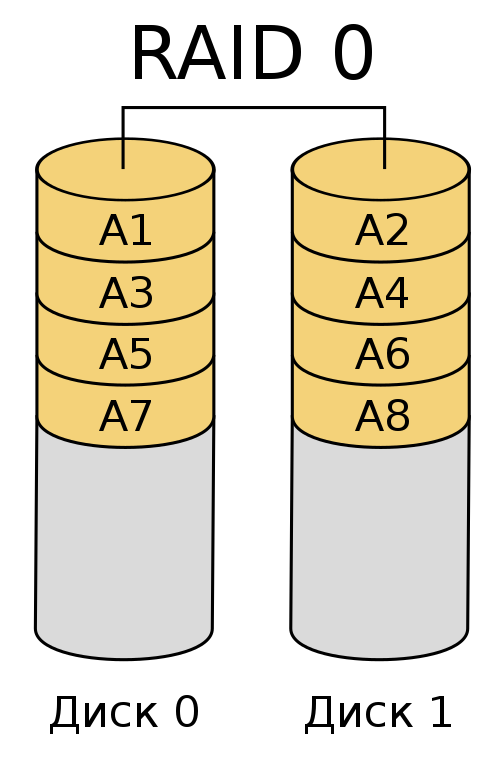
\includegraphics[width=0.4\linewidth]{10/0}}
\end{minipage}
\hfill
\begin{minipage}[h]{0.49\linewidth}
\center{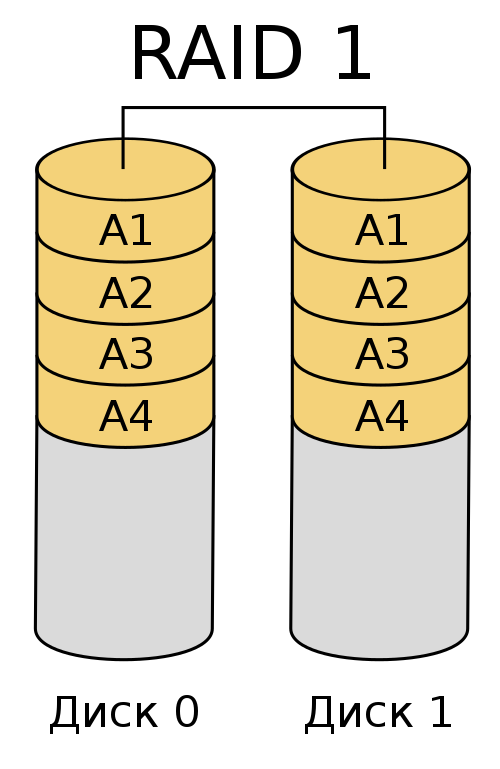
\includegraphics[width=0.4\linewidth]{10/1}}
\end{minipage}
\end{figure}

RAID 1. \\
массив из двух (или более) дисков, являющихся полными копиями друг друга. (Все диски объединяются в пары и дублируют информацию)
Главный недостаток этого подхода, это то что при формальном количестве $2n$ дисков пользователь получает только $n$

RAID 2. \\
На лекции про него не говорили. Там используются контрольные суммы с помощью кода Хемминга. В настоящее время нигде не используется. 

RAID 3. \\
Вспомним для начала, что такое XOR (исключающее ИЛИ, оно же сложение по модулю 2). Главное свойство этой операции в том, что если 
$a \oplus b = c$, то $c \oplus b = a$ так как $(a \oplus b) \oplus b = a \oplus (b \oplus b) = a$ (c b аналогично). \\
Применим эту идею. Разделим информацию на блоки (Если следовать картинке) $A_1, A_2 ... A_6, B_1, B_2 ... B_6$. На первые три диска последовательно запишем блоки информации, а на последний $A_1 \oplus A_2 \oplus A_3$, $A_4 \oplus A_5 \oplus A_6$ и т.д. Тем самым, если выйдет из строя диск 2, то с помощью рассмотренного выше свойства получим утерянную информацию. Главный недостаток - может сгореть диск с XOR других дисков (на картинке это Диск 3)

\begin{figure}[h!]
\begin{minipage}[h]{0.49\linewidth}
\center{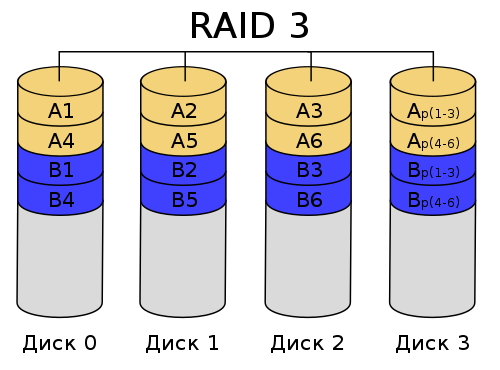
\includegraphics[width=0.5\linewidth]{10/3}}
\end{minipage}
\hfill
\begin{minipage}[h]{0.49\linewidth}
\center{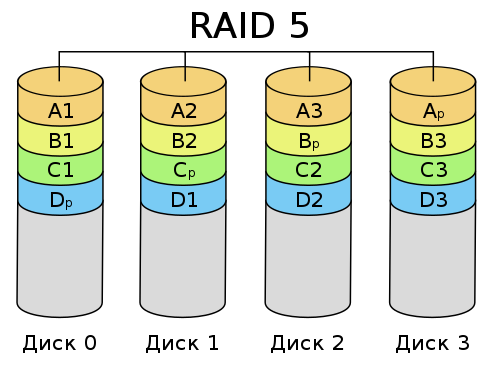
\includegraphics[width=0.5\linewidth]{10/5}}
\end{minipage}
\end{figure}


RAID 4. \\
Очень похож на RAID 3, больше про него на лекции ничего не сказали.

RAID 5.
Та же идея что и в RAID 3, только результат исключающего ИЛИ хранится не на одном конкретном диске (он ведь тоже может сгореть !) а на всех. Например, информация разделена на блоки $A_1, A_2, A_3, B_1, B_2, B_3, C_1, C_2, C_3, D_1, D_2, D_3$, так же:
$A_p = A_1 \oplus A_2 \oplus A_3$, 
$B_p = B_1 \oplus B_2 \oplus B_3$ аналогично для $C, D$. Тогда на дисках все будет выглядеть как на картинке. (Остается добавить, что в случае RAID 3 все блоки информации $A_p, B_p, C_p, D_p$ хранились бы на 3 Диске)

\url{https://ru.wikipedia.org/wiki/RAID}

\subsection {Распределение данных}

\begin{itemize}
\item горизонтальное распределение, когда распределяются данные одного типа. Например, в БД "студенты" данные студентов МГУ хранятся на узле в Москве, а данные студентов СПбГУ - в Санкт-Петербурге. 

\item вертикальное распределение, когда распределяются данные разных типов. Например, в учебной части хранятся оценки, а на кафедре физ.воспитания спортивные достижения. 

\item дублирование (т.е. подразумевается непрерывная передача данных между, например, двумя базами) Различают два типа дублирования - синхронное и асинхронное. Про каждый из них ниже
\end{itemize}

Синхронная передача данных \\
Синхронную передачу применяют в случае, когда базы находятся рядом друг с другом. Принцип работы заключается в том, что каждая запись одной базы пересылается на другую с помощью двухфазного коммита. 
Модель двухфазного коммита
\begin {itemize}
\item Пользователь заходит на сервер I и делает изменения на сервере I и на сервере II
\item Пользователь решает зафиксировать свои изменения (операция commit). Сервер I отправляет запрос на сервер II может ли он зафиксировать изменения.
\item Если сервер II отвечает нет (не может зафиксировать), то изменения не фиксируются. Иначе сервер I коммитит изменения у себя и отправляет сообщение серверу II, чтобы он тоже закоммитил изменения у себя. 
\item Сервер II отвечает об успешной фиксации изменений
\end {itemize}


Асинхронная передача данных \\
В случае, когда серверы находятся далеко друг от друга пользователь каждый раз при коммите будет долго ждать пока запись "дойдет" до второго сервера. Поэтому используется следующий подход. 
\begin {itemize}
\item Клиент зашел на сервер I и сделал какие-то изменения.
\item Эти изменения не отправляются на сервер II, а пишутся в специальный "журнал" на сервере I, в котором хранится только то, что изменилось и где. 
\item Как только сервер I записал изменения в журнал, пользователь получает сообщение, что изменения закоммичены. 
\item Специальный процесс, отправляет на сервер II журнал (например, когда он будет полностью заполнен, хотя может отправлять и чаще). \item Передача данных завершена 
\end {itemize}